\newpage
\section{Корректировка бизнес-процессов}
Рассмотрим процесс мониторинга в контексте будущей системы (рисунок
\ref{ris:to_be_main_view}).

\subsection{Составляющие процесса мониторинга}

\begin{figure}[h]
\center{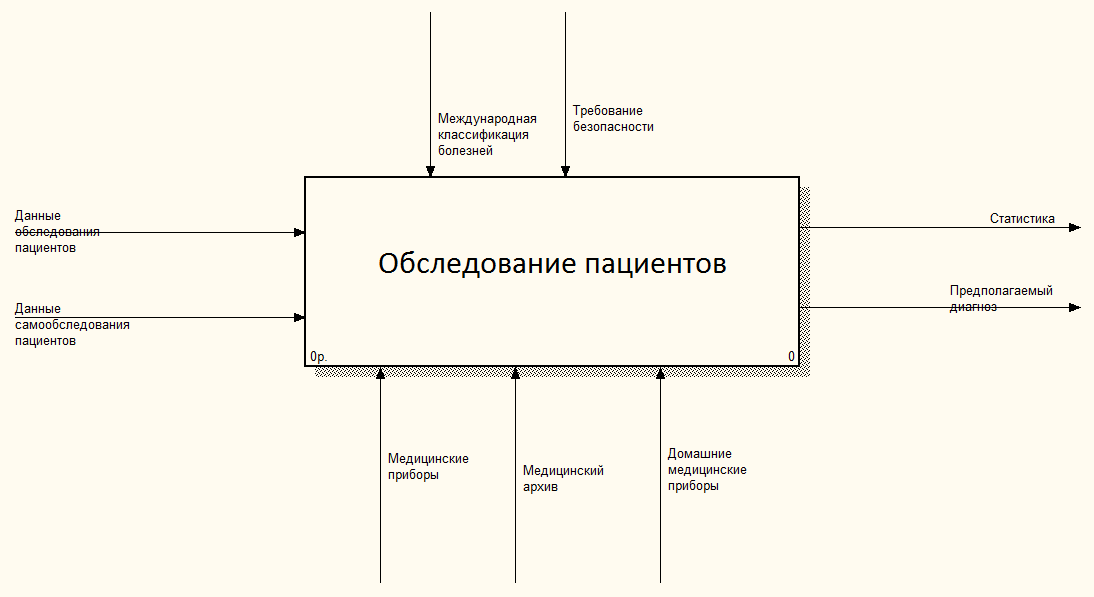
\includegraphics[width=1\linewidth]{to_be_main_view.eps}}
\caption{Общая схема мониторинга}
\label{ris:to_be_main_view}
\end{figure}

Единственным объектом исследования в системе является - обследуемый пациент. Система должна вести постоянный мониторинг и анализ состояния пациента.
Для получения данных о пациенте и их анализа могут быть использованы:

\begin{enumerate}
  \item Медицинские устройства. К ним относится аппараты, расположенны в
  лечебном учреждении и находящиеся в общем доступе для всех пациентов. К ним можно отнести рентген-установка, МРТ-сканер, УЗИ, тонометры, термометры, пульсметры и другие.
  \item Персональные устройства мониторинга. К ним можности приборы, доступные
  для использованиии в домашних условиях, а именно: электронные тонометры и термометры. Помимио этих приборов существуют так называемы комплексные датчики предназначеные для пользователей, не являющихся специалистами в области сердечно-сосудистой диагностики. К таким приборам относится Ангиоскан-01М (Персональная версия) – предназначен для работы под управлением персонального компьютера. Данный прибор надевается на палец пациента и устанавливает подключение к персональному компьтеру или ноутбуку. Прибор позволяет измерять следуюущие показатели: частоты сердечных сокращений; жесткости сосудов; типа пульсовой волны; биологического возраста сосудов; индекса сатурации (насыщение гемоглобина кислородом); уровня стресса.
  \item Сервер с необходимым програмным обеспечением. На нем будет развернута
  база данных, в которой будут храниться персональные данные всех участников системы,медицинская информация пациентов и прочие информационные объекты, котоыре будут определын ниже,  в разделе Концептуальная модель предметной области. Также на сервере будет находиться веб-интерфейс системы, доступный пользовтаелям.
\end{enumerate}

Процесс мониторинга должен соответствовать определенным стандартам и законодательным актам.

Контролировать процесс должен лечащий врач или врач, непосредственно, осуществяющий оказание той или иной услуги пациенту.

Результаты процесса мониторинга представляются в виде различного рода отчетов.

\subsection{Основные этапы процесса мониторинга}

\subsubsection{Регистрация в системе}

Этап предназначен для создания учетной записи пациента при обращении в данное
лечщее учреждение впервые. С данной учетной записью будут соотносится данные,
полученные в процессе лечения, обследований. Важно чтобы продолжительность
данного этапа была минимальной, а процедура регистрации максимально простой,
чтобы процесс обследования пациента начался максимально быстро.
Возможны два варианта регистрации пациента в системе:

\begin{enumerate}
  \item Самостоятельная регистрация. Данный вариант подходит для иногородних
  пациентов.
  \item Регистрация при посещении лечащего учреждения.
\end{enumerate}

После прохождения процедуры регистрации пациент может быть записан на первичный
прием к врачу.

\subsubsection{Первичное обследование}

На первичном приеме врач формирует электронную карту обследований, которые
необходимо пройти пациенту для оценки состояния здоровья. Факторами влияющими на
набор обследований который должен пройти пациент являются:
\begin{enumerate}
  \item Устные показания пациента
  \item Больничная карта пациента
  \item Опыт врача   
\end{enumerate}

Во время первичного приема у врача начинается непостредственный постоянный
мониторинг за состоянием пациента.

После составления карты обследования пациент проходит первичное обследование.
Первичное обследование необходимо для формализации состояния пациента на момент
обращения в лечащее учреждение. Оценка состояния пациента, полученная в
результате первичного обследования будет учитываться в показателях оценки
эффективности лечения.

\subsubsection{Лечение}
После прохождения пациентом первичного обследования формируется план лечения
пациента. План лечения пациента может быть многоэтапным. После завершения
каждого этапа происходит оценка эффективности лечения.

План лечения на каждом этапе может включать в себя:

\begin{enumerate}
  \item Режим дня пациента
  \item Режим приема лекарственных препаратов
  \item Расписание приемов
  \item Расписание обследований    
\end{enumerate}

Основной задачей системы на данном этапе является ослеживание качественных и
количественных показателей состояния пациента.

\subsubsection{Мониторинг}
Процесс мониторинга является “сквозным” и присутствут на многих этапах. Основной
задачей процесса является сбор данных в процессе лечения и обследований
пациента.
Основными процессами в результате которых в систему попадают данные о пациенте
являются:

\begin{enumerate}
  \item Прием у врача
  \item Стационарное лечение
  \item Обследования
  \item Амбулаторное лечение 
\end{enumerate}

Основными источниками даных о пациенте являются:

\begin{enumerate}
  \item Результаты обследований
  \item Результаты анализов
  \item Результаты осмотров у врача
  \item Устные показания пациента
  \item Показания врача 
\end{enumerate}

Основные способы внесения данных в систему:

\begin{enumerate}
  \item Ручной ввод
  \begin{enumerate}
    \item Ввод данных пациентом
    \item Ввод данных врачом
  \end{enumerate}
  \item Автоматический ввод данных медицинскими устройствами
\end{enumerate}

\subsubsection{Накопление данных}
Процесс заключается в сохранении поступающих в систему данных для их последующей
обработки и анализа.

\subsubsection{Анализ данных}
Объем данных, поступающих в систему достаточно большой. Для ускорения обработки
данных их необходимо анализировать. Согласно требованиям к системе, процесс
анализа данных включает в себя:

\begin{enumerate}
  \item Оценку эффективности лечения
  \begin{enumerate}
    \item Оценки влияния лекарственных препаратов
    \item Оценки влияния процедур, операций 
  \end{enumerate}
  \item Получение отчетов. Отчеты представлены в виде:
  \begin{enumerate}
    \item Агрегированные данные
    \item Рекомендации по лечению
  \end{enumerate}  
\end{enumerate}










